\documentclass{article}
\usepackage{graphicx}

\begin{document}

\begin{titlepage}
\title{ECS189G Homework 2 Report Problem B}
\author{Goh Chang Kang, Charles 916751838, \\
Yang Minxing 916751773, Chen Jieyi Chloe 999823783}

\date{October 30, 2018}
\maketitle
\end{titlepage}


\section{Background}

In the ivl data set, the user and item ID indicates the identity of a user and a professor. We cannot assume that they are consecutive because there may be some user or item ids that are missing. For example I could have user ids 1, 2, and 4. This would mean I am missing id 3. This is apparent in the dataset when we check the maximum item ID vs the number of unique IDs

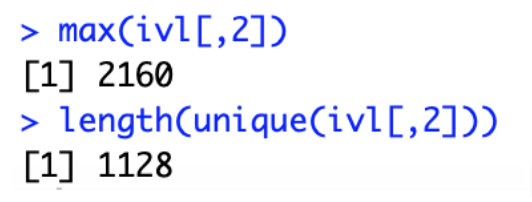
\includegraphics[scale=0.5]{NonConsecutiveIDExample.png}

We can also see this during the matrix factorisation process. When the matrix is split into its component vectors P and Q, the former representing users and the latter representing items, we see that actually the Q matrix is not full rank and contains many NaN values.  This will cause problems when multiplying, and would also cause problems during computation since in R any operation on NaN returns a NaN value

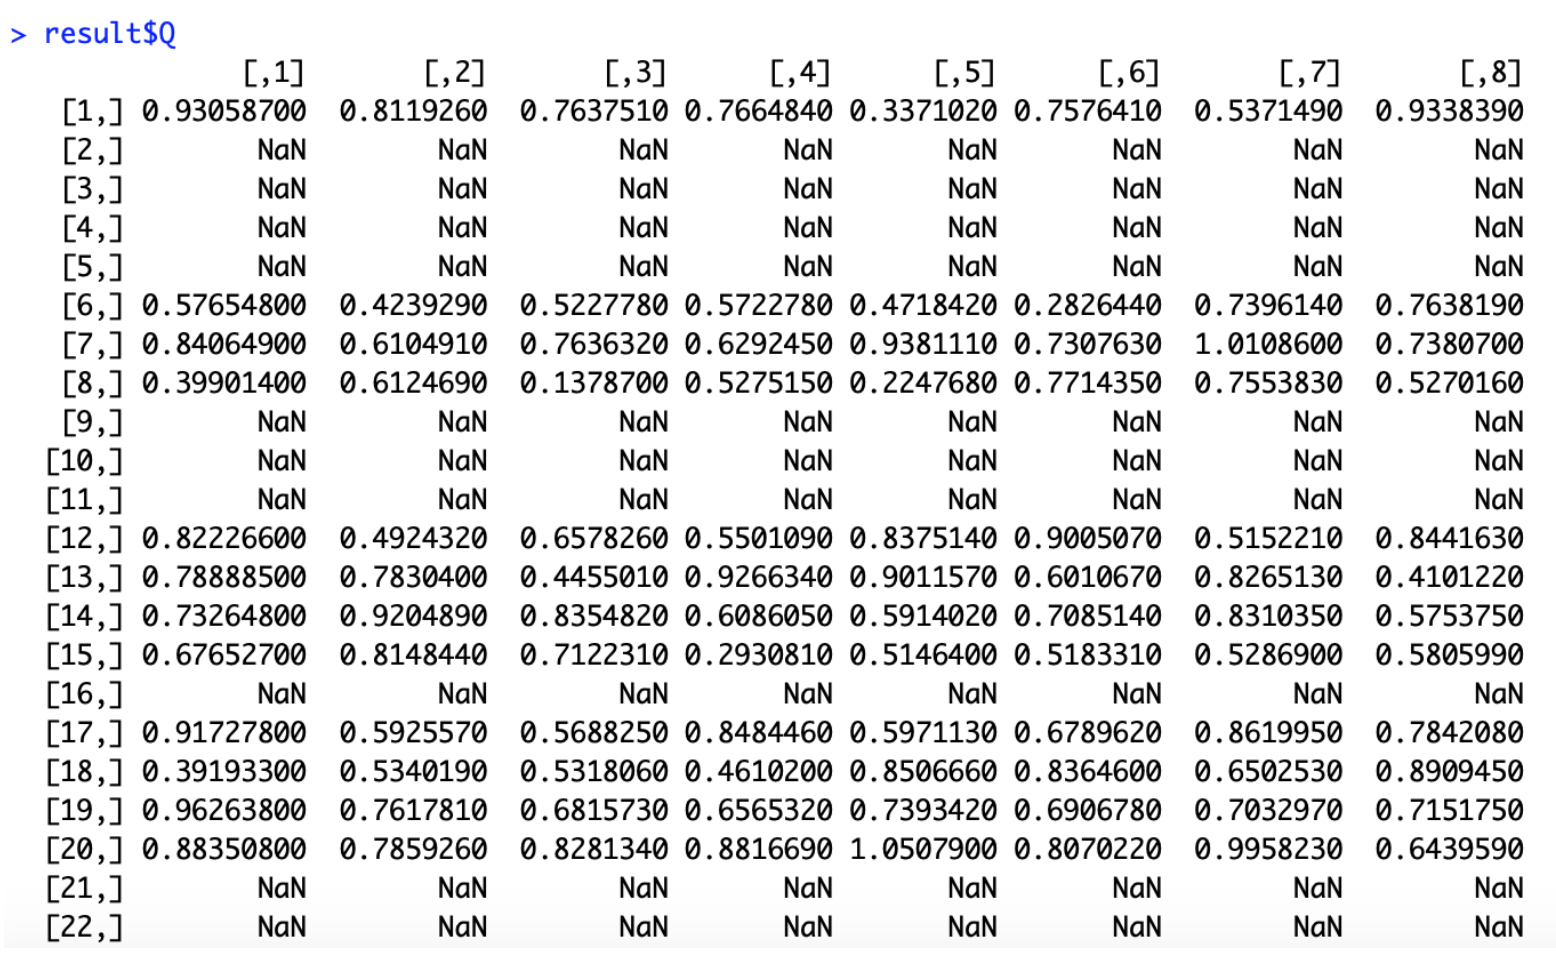
\includegraphics[scale=0.4]{ItemIDMissingExample.png}

To solve this problem, we made changes to the trainReco() function as well as the predict() function

\section{Changes to trainReco()}

For the purposes of simplicity, the changes for the function when dealing with item id will be described.  The same changes are made when dealing with user id. For item id, we take the maximum id and the number of unique ids. If they are equal, we do not need to rectify it. If they are not equal, that means there are non-consecutive item ids. We then compress the ids into consecutive ones without changing the relative position in the table. Finally at the end of the function we added a translator dataframe to our output result. This will serve as the translator of original id to translated id in the predict function. 

\begin{verbatim}
library(rectools)
trainReco <- function (ratingsIn, rnk = 10, nmf = FALSE) 
{
  require(recosystem)
  hasCovs <- (ncol(ratingsIn) > 3)
  if (hasCovs) {
    covs <- as.matrix(ratingsIn[, -(1:3)])
    lmout <- lm(ratingsIn[, 3] ~ covs)
    minResid <- min(lmout$residuals)
    ratingsIn[, 3] <- lmout$residuals - minResid
  }
  #check for consecutive records.
  #if the max ID is greater than the num of rows, means they are not consecutive
  sMax <- max(ratingsIn[, 1])
  sUnique <- length(unique(ratingsIn[, 1]))
  sOriginal <- ratingsIn[, 1]
  
  dMax <- max(ratingsIn[, 2])
  dUnique <- length(unique(ratingsIn[, 2]))
  dOriginal <- ratingsIn[, 2]
  
  #if they are not consecutive, we use the shrinked ones
  if ((sMax - sUnique) > 0) {
    sortedIdx <- sort(unique(ratingsIn[, 1]))
    sIDTemp <- match(sOriginal, sortedIdx)
    #use the relative position as the new ID, because positions must be consecutive
  } else {
    sIDTemp <- sOriginal
  }
  
  if ((dMax - dUnique) > 0) {
    sortedIdx <- sort(unique(ratingsIn[, 2]))
    dIDTemp <- match(dOriginal, sortedIdx)
  } else {
    dIDTemp <-dOriginal
  }
  
  r <- Reco()
  train_set <- data_memory(sIDTemp, dIDTemp, 
                           ratingsIn[, 3], index1 = TRUE)
  r$train(train_set, opts = list(dim = rnk, nmf = nmf))
  result <- r$output(out_memory(), out_memory())
  attr(result, "hasCovs") <- hasCovs
  if (hasCovs) {
    attr(result, "covCoefs") <- coef(lmout)
    attr(result, "minResid") <- minResid
  }
  class(result) <- "RecoS3"
  #append the attribute for translation purpose
  result$translator <- data.frame(sIDTemp, dIDTemp, sOriginal, dOriginal)
  result
}
\end{verbatim}

\section{Changes to predict.RecoS3()}

In the predict.RecoS3 function, we grab the appended translator dataframe and search for the translated id in the compressed version using the inputted id (which is the original reference).

\begin{verbatim}
predict.RecoS3 <- function (recoObj, testSet) 
{
  p <- recoObj$P
  q <- recoObj$Q
  testSet$pred <- vector(length = nrow(testSet))
  hasCovs <- attr(recoObj, "hasCovs")
  if (hasCovs) {
    covCoefs <- attr(recoObj, "covCoefs")
    minResid <- attr(recoObj, "minResid")
  }
  for (i in 1:nrow(testSet)) {
    j <- testSet[i, 1]
    k <- testSet[i, 2]
    #use the translator to translate to consecutive ID
    originalSIndex <- match(j, result$translator[[3]])
    originalDIndex <- match(k, result$translator[[4]])
    j <- result$translator[[1]][originalSIndex]
    k <- result$translator[[2]][originalDIndex]
    if (!is.na(j) && !is.na(k) && j <= nrow(p) && k <= nrow(q)) {
      tmp <- 0
      if (hasCovs) 
        tmp <- covCoefs %*% c(1, testSet[i, -(1:3)]) - 
          minResid
      testSet$pred[i] <- p[j, ] %*% q[k, ] + tmp
    }
    else testSet$pred[i] <- NA
  }
  testSet$pred
}
\end{verbatim}

Note: We also added an extra check for non-existing values when predicting (as quoted below):

\begin{verbatim}

if (!is.na(j) && !is.na(k) && j <= nrow(p) && k <= nrow(q))

\end{verbatim}

After fixing the non-consecutive id problem, we can re-check our matrix-factorisation components and see that there are no more NaN values, thus confirming that we have indeed compressed the ids successfully.

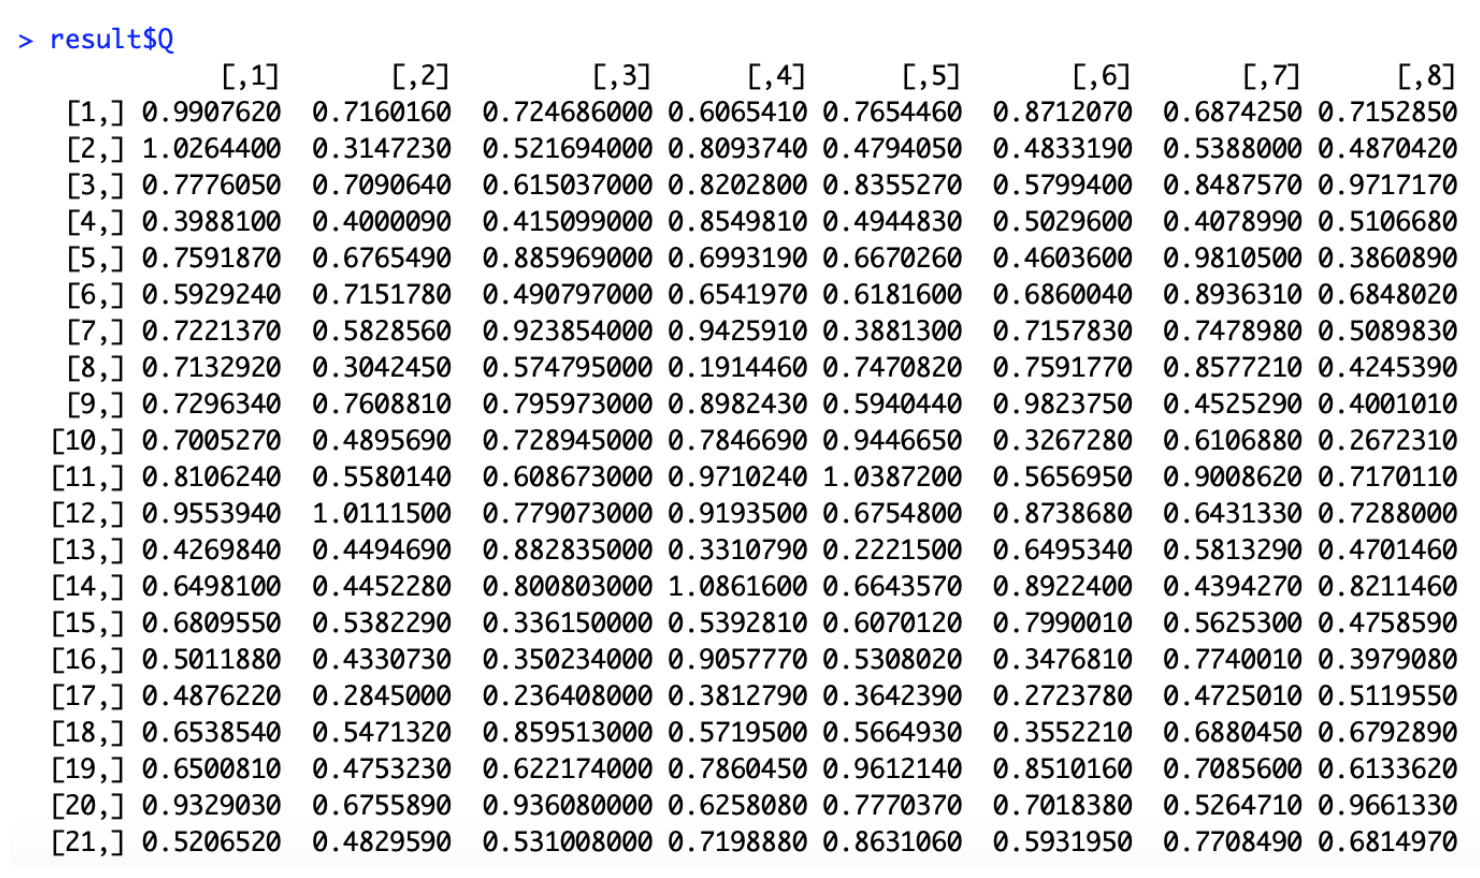
\includegraphics[scale=0.5]{ItemIDFixedExample.png}

\end{document}